\documentclass{sig-alternate-05-2015}
\usepackage{float}
%\usepackage{enumitem}
\usepackage{subfiles}
\usepackage[english]{babel}
\usepackage{graphicx}
\usepackage{epstopdf}
\usepackage{tabularx}
\usepackage{url}
\usepackage{xcolor}
\usepackage{soul}

\makeatletter
\def\@copyrightspace{\relax}
\makeatother

\begin{document}
\title{A user interface for terrain modelling in a VE using a head mounted display}

\numberofauthors{1}
\author{
\alignauthor
Timothy Gwynn\\
       \affaddr{GWYTIM001}\\
       \affaddr{University of Cape Town\\
       Supervisor: J. Gain}
}
\maketitle
\begin{CCSXML}

\end{CCSXML}



\printccsdesc
%\keywords{Virtual Environments, Terrain Synthesis, User Testing}

\section{Introduction}
To aid in the creation of 3D terrains for virtual environments(VEs) we look at the effectiveness of designing terrains using VE technology. VE design tools allow designers to work in the same medium as the content consumers and to avoid some of the challenges characteristic to creating 3D content using 2D interfaces.\\

Terrain modelling is a method for creating realistic virtual landscapes. It allows the designer to set constraints in order to shape the terrain as desired. A synthesis application will then attempt to create a realistic terrain based on these restraints. In this way the designer can create terrain with specific global and local features without manually editing every detail. The terrains can then be used as components for natural environments in computer games, films and simulation and training scenarios\cite{Gain2015}

\begin{figure}[H]
	\centering
	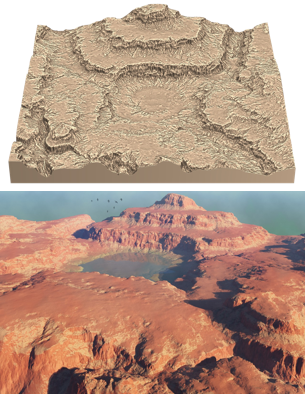
\includegraphics[width=5cm]{Terrain2}
	\caption{A synthetic terrain}
\end{figure} 
VEs describe a set of three dimensional visual input and output technologies which aim to embed users visually within virtual worlds. They can be thought of as the visual equivalent of technologies such as surround sound or headphones. CAVE (CAVE Automatic Virtual
Environment) surrounds the user with a number of large screens and also tracks user head position\cite{Cruz-Neira1993} providing the visual equivalent of surround sound. HMD devices fit over the user's face and the device itself is tracked and can be described as headphones for your eyes.\cite{Alger2015}

VE technologies are also often associated with novel input devices such as 6 degree of freedom(DOF) devices, which allow users to provide 3 dimensions of positional input and 3 dimensions of rotational input. Unlike traditional WIMP (windows, icons, menus, pointer) interfaces, where almost every system is designed for a mouse and keyboard, VE systems tend to rely on specialized input devices\cite{Hand1997,Bowman2001}. Because of this there are already a wide range of input devices, resulting in few general standards for interface design. However, with the recent increase in consumer access to commercial devices such as the Oculus Rift and HTC Vive, that come with generic controllers this may soon change.\\

To determine the potential of using VEs for terrain modelling  we must look at terrain synthesis, VE interface design for 3D modelling and previous research comparing desktop and VE systems. Using VEs with 6-DOF devices has proven to be more efficient than WIMP interfaces for basic object manipulation\cite{Schultheis2012,Scali2003}. Although more complex systems have been implemented there has been little objective evaluation of them although subjective evaluations are generally positive\cite{Wang2013,Mine2014,Jerald2013}. Post-WIMP interfaces promise a radical change in the way we interact with software applications and, if implemented well, could result in greatly increased productivity and control using VEs.
 
By creating VE systems for designers to perform terrain modelling we allow them to better understand and design experiences for VEs. Additionally, we hope to provide a design environment that is more efficient than a desktop system for experienced users. Due to the potential for increased immersion and flow in VEs compared to desktop environments\cite{Schubert2001} we also hope to encourage these phenomena in the design workflow.
\section{Background}
There are large bodies of work on both interactive terrain synthesis and VE interface design. However, it should be noted that work related to terrain synthesis tends to focus on the synthesis techniques rather than the interface. Additionally, most VE interfaces use custom or specialized controllers and other hardware. Earlier works, in particular, discuss issues such as motion sickness, which modern hardware has largely solved.
 
Here we detail current solutions to interactive terrain synthesis and a range of interface design techniques for 3D modelling in VEs. We also cover work on tasks that can be accomplished more quickly in VEs than on desktop systems. This provides one of the primary motivations for our research. Finally, we discuss previous systems that were designed to do similar VE modelling tasks.
 
\subsection{Terrain Synthesis} 
Virtual landscapes are an important component in representing natural environments for applications such as computer games, film, simulation and training\cite{Gain2015}. Therefore, fast and realistic terrain synthesis has been the subject of considerable study with a variety of techniques such as patch or texture-based synthesis\cite{Cruz2015, Tasse2012}, noise-based synthesis\cite{Musgrave1989} and erosion simulation\cite{Anh2007}. With advances in graphics processing technology we are now able to simulate terrain that is indistinguishable from real terrain examples\cite{Gain2015}. 

Gain et al.'s terrain synthesis system allows users to introduce constraints into the terrain synthesis process using a number of tools\cite{Gain2015}. The ability to add and modify constraint points and curves to a landscape allows users to create landscape features such as hills, ridges and valleys. Type constraints can be painted onto the landscape to define areas of a certain type such as `swamp', `dirt', etc. To implement these constraints users have access to a combination of sketching, painting and 3D widget interface elements.

\begin{figure}[H]
	\centering
	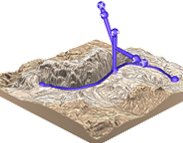
\includegraphics[width=6cm]{Terrain1}
	\caption{An example of the 3D widgets}
\end{figure} 

Another terrain editing system presents a sketch based technique which allows users to  edit terrain from first person point of view\cite{Tasse2014}. Users are able to sketch a horizon shape which the system then uses to create a number of constraints which the synthesis process must obey.
\subsection{Interface design for modelling in large-scale Virtual environments}
When designing an interface for modelling in large-scale VEs there are three important aspects to consider: User navigation and movement, Interface interaction and Environment interaction\cite{Bowman2001}. Respectively, these allow the user to move within the VE, select their mode of interaction and interact with the VE. Below we look at each of these aspects in detail and some of the successful, and unsuccessful, interface implementations in each area.
%\hl{Somewhere need to talk about camera control, not sure where cite ware and bowman}
\subsubsection{Navigation in Virtual Environments}
A common problem for users in VEs is becoming disorientated and lost within the VE\cite{Darken1993}. This may be due to a number of issues such as the user being unfamiliar with the environment or not having sufficient location and orientation information available. Below there are some examples from research that aims to solve the problem of effective navigation and travel in VEs.\\

As landmarks are commonly used in everyday scenarios that require navigation there has been considerable research into effectively using them within VEs.

For example, research has been done to establish whether users orientate themselves via local or global landmarks\cite{Steck2000}.It was found that users do not consistently use a single type of landmark. However, users rarely used both local and global types simultaneously. This suggests that users tend to use the most visually distinct land marks and will prefer to use landmarks that are not occluded. A good example of this would be a static sun-like object in the sky. %This implies that for navigation, interface design should provide a variety of landmarks, both global and local, that allow the user to always have a distinctive point of reference. It also suggests that global landmarks that will not be occluded by local geometry should be used. 

Further research into the design of landmarks for VEs found that in natural environments users tend to use landmarks that resemble man-made artefacts\cite{Vinson1999}. Additionally it was suggested that landmarks should all be orientated the same way and marked according to this orientation. This allows the user to extract orientation information as well as location information from a single landmark.\\

Another study compared a variety of tools for navigation in VEs including landmarks, breadcrumb markers and maps, amongst others\cite{Darken1993}. They associated their techniques with natural human and avian  navigational behaviours. They found that the map view in particular allowed for straightforward navigation although they suggested that this was linked to the navigation space being a 2D plane. Where users could fly vertically, letting them observe the navigational space from above, they were also able to follow a simple sequence of actions for accurate navigation. They also found that, while landmarks were effective for distinguishing certain areas they provided little directional information. When they added a synthetic sun and shadows in the test case with landmarks they found that user performance increased significantly. %While they did not evaluate the effectiveness of the different techniques they did detail the common behaviour of the test subjects for each technique. By observing which techniques lead to simple or complex behaviour we can surmise which techniques are effective from an ease of use perspective.

These results reinforce the concept of a combination of local and global landmarks being useful for navigation\cite{Darken1993}. Additionally, the ease of use of both the map and the flying technique suggest that allowing the user to move in 3 dimensions and providing a map will aid navigation considerably. We suggest that in a 3D environment where 3D movement is possible a 3D map is better suited to aiding navigation. This will allow the user to read their height directly from the map and possibly aid the user in determining the scale of objects.\\

Although having effective navigation techniques is important they are useless without some method of travel. Bowman et al. have created a list of aims for effective travel techniques.\cite{Bowman1997} These include, speed, accuracy, spatial awareness, ease of learning, ease of use, information gathering and presence. We suggest that user comfort should also be taken into account especially when designing a VE interface for 6-DOF controllers.

 In the same paper travel techniques are categorized into two groups: Gaze directed steering and gesture directed steering\cite{Bowman1997}. Gaze directed steering refers to instances where the user's navigation is controlled via a tracked HMD while gesture directed  steering involves the user controlling their direction of movement through gestures (with or without props).Their findings suggest that gesture directed steering would be more appropriate in our context according to the aims stated above.
 
 %Bowman et al. then performed a series of experiments where they found that tool directed navigation was faster than gaze directed navigation for navigating relative to objects and equal for navigating to an absolute point in space. Additionally since gesture directed steering allows the user to freely observe their environment during travel it allows for superior spatial awareness and information gathering. We therefore suggest that we should prefer gesture directed steering techniques.


\subsubsection{Interface interaction in VEs}
 Interface interaction refers to the user modifying the state of the system or the mode of interaction\cite{Bowman2001}. Typical examples of this include menu interaction and tool selection. These tasks, which are often 2D or 1D in nature are ill suited to 3D environments \cite{Bowman2001, Hand1997}. In particular, the increased dimensionality of the task can lead to a significantly higher error rate and issues of occlusion need to be considered\cite{Hand1997}.
 
Therefore we must consider novel interface elements. For example, a ``ring menu" is a way to implement 1D interface interactions that allow users to navigate menus or select tools\cite{Hand1997}. Other alternatives to traditional menu interaction include gesture-based shortcuts\cite{Zeleznik2007} or speech input \cite{VanDam1997,Bowman2001,Hand1997}. Additionally, combinations of interaction methods can be used. For example, gesture-based shortcuts and radial menus can be combined to allow users utilize muscle memory to select tools from the radial menu using gestures without actually displaying it.\cite{Kurtenbach1993}\\
 
 An element of interface interaction to be considered is ``clutching", where a user must pause movement tracking so as to reset to a comfortable position\cite{Hand1997}. Importantly, this needs to be done without interfering with the current interaction. For example, when a user intends to rotate an object further than is comfortable with a single movement. Typically this can be done by providing the user with a button to toggle motion tracking on and off. However, this is annoying for the user and feels unnatural\cite{Hand1997}.  A suggested solution is to utilize a direct mapping of controls onto virtual objects combined with two-handed-interaction(THI). This can reduce or remove the need for artificial clutching mechanisms\cite{Hand1997}.  Hinckley et al. suggest that utilizing THI can reduce the need for clutching by tracking gestures of the dominant hand (DH) relative to those of the non-dominant hand (NDH)\cite{Hinckley1994}. They also suggest that an alternative is to use a physical 3D prop such as those used by Ware et al. for there eye-in-hand metaphor\cite{Ware1990}.\\
 
 The depth positioning of interface elements is another challenge in VR that is simply not present in desktop systems.\cite{Alger2015} This is because HMD devices use stereoscopy to create depth, traditional desktop systems do not have this issue as all interface elements must be placed on the 2D screen. Therefore, we need to avoid having interface elements that are too close to the user in the visual field, so that they are hard to focus on or having elements that are out of comfortable reach. These constraints combine to leave a somewhat restricted area in which to place interface elements.
 
As well as considering where interface elements are placed in the virtual space we also should provide users with indications of where objects in their physical environment are. This helps reconcile the differences between the virtual reality a user is immersed in and their surroundings\cite{Duval2014}. Reasons to show some of the user's physical environment include: allowing them to more easily interact with physical devices such as keyboards and other objects, preventing inadvertent physical contact which may cause injury or distraction and being able to interact with other people without exiting the VE completely.
 
\subsubsection{Environment interaction in VEs}
 Interaction with the environment involves the user making changes to the virtual world through selection and manipulation of objects. To do this users should, at a minimum, be able to either select, position or rotate objects\cite{Bowman2001}. Research in this area addresses both the wide range of hardware devices created for interacting with VEs as well as related software solutions. Common tools include a motion-tracked glove \cite{Zimmerman1986}, spaceballs\cite{Hand1997}, and pen or wand controllers\cite{Schultheis2012}. As opposed to WIMP interfaces interaction with VEs is often based on direct manipulation where the user 'grabs' an object and then manipulates it as one would manipulate a malleable physical body.
  
 In this area considerable research has gone into establishing the advantages of THI over other interaction methods. It is widely agreed that humans are better able to judge the relative, rather than absolute, position of their hands \cite{Bowman1998, Buxton1986}. Additionally, users have a preference for THI\cite{Buxton1986} and perform certain basic manipulation tasks such as rotation and translation more efficiently when using two hands\cite{Schultheis2012,Balakrishnan1999}. Therefore interfaces should be designed for bi-manual interaction and motion should be tracked with the DH relative to the NDH\cite{Hinckley1994}.\\
 
 Another area of interest in environment interaction is how to interact with objects far away from the user. This is commonly referred to as action at a distance (AAAD). This would be necessary for our interface to allow users to manipulate points in the terrain that are far away from the users viewpoint. Techniques to address this include the go-go hand technique\cite{Poupyrev1996}, where the hand is tracked and then non-linearly mapped into the VE and a number of ray-casting techniques \cite{Bowman2001}. These methods roughly correspond to the function of a cursor in a 2D environment. Hand et al.\cite{Hand1997} suggest that although cursors are a necessary metaphor in a 2D environment they do not correspond well with natural gestures for use in VEs.
 
 Although there are a number of ways to perform AAAD users also need depth cues to manipulate or select objects with precision.\cite{Schultheis2012} Some suggested methods for this include representing the user's hand as a transparent outline in the VE\cite{Hinckley1994}, drawing a line between the user's hands in the VE\cite{Schultheis2012} or creating a plane of action\cite{Mine2014} on which the user acts. To further simplify environment interaction, particularly when working with stereoscopic depth, studies suggest that interactive DOF should be restricted as much as possible\cite{Bowman2001}.

\subsection{Comparison of Desktop applications to Virtual environments}
The primary motivation for designers to adopt a VE based workflow is to achieve increased productivity. Therefore, it is important to consider areas in which VE systems perform significantly better than traditional desktop systems.Fortunately, there have been a number of studies comparing user performance in VEs and desktop environments.\\

VE systems have been shown to be particularly effective for simple object manipulation. Studies have shown that expert users are able to complete simple tasks up to 8 times faster in the VE than on a desktop\cite{Schultheis2012}. However, in more complex applications, especially where indoor navigation was required, users tended to perform better on desktop systems\cite{SousaSantos2009}. Additionally, from a number of previous experiments it is evident that the amount of training users receive has a significant impact on results. Despite this, even users with little training report that the VE interfaces were more intuitive and easier to use than desktop systems, even when other measures showed no significant difference in task performance.\cite{Toma2012}.

Some of the most detailed data regarding task performance in VEs comes from an experiment comparing a traditional WIMP interface to a number of VE set-ups. Each VE system tested featured THI with 6-DOF controllers. However, the researchers varied the presence of stereo-vision, haptic feedback and a snapping tool\cite{Scali2003}. Users performed a series of tasks that involved translating, rotating and scaling objects to fit onto pre-defined surfaces. They found that the VE systems outperformed the WIMP interfaces with regards to time for task completion, perceived workload and usability. Additionally they found that although haptics and stereo vision did not significantly affect task completion times, haptics had a significant effect on perceived workload and usability.


\subsection{Designing for Virtual Environments in Virtual Environments}
It is only in recent years that the technology for effectively creating content in VE systems has become available. However, there are already a variety of systems for modelling 3D objects and environments in VEs. Additionally, early research into the design of VE systems revealed some basic principles that can be incorporated into modern systems. By looking at solutions in existing systems and incorporating general VE design principles we can address some of the common problems inherent to working with VEs.\\

From early research into THI it was found that people have an instinctive awareness of the relative position of their hands\cite{Bowman1998, Buxton1986}. Some modern systems take advantage of this to solve the issue of 2D menu depth in a scene by implementing systems such that the menu is attached to the user's NDH either as a physical touch screen\cite{Wang2013,Mine2014} or as a virtual representation\cite{Jerald2013}. Because the menu is always at a constant position relative to the user's NDH they are able to reliably interact with it using their DH.

Although THI systems that use 6-DOF devices have been shown to increase performance with regards to interaction speed\cite{Schultheis2012} they often induce fatigue in users. For example, in an experiment where a handlebar metaphor was used to control the camera users consistently reported feeling fatigued\cite{Song2012}. However, from previous experiments we observe that bringing geometry to the user instead of making the user reach out to the geometry provides an experience with very few fatigue issues\cite{Jerald2013}.

Another problem related to using 6-DOF devices is the difficulty of incorporating textual and numerical input. To address this, a number of systems incorporate a form of voice input to make up for the absence of a keyboard\cite{Ponto2013,Toma2012}. An implementation of this in the \textit{Placeholder} system\cite{Laurel1994} allows users to create audio notes at certain locations that would be recorded and then could be played back at any time.

Modern VE systems that incorporate THI for 3D modelling suggest keeping the functions of each controller relatively independent\cite{Mine2014}. For example, using the NDH to control movement while the DH is used for interacting with the environment. This means that users do not have to use both controllers for every action. This seems to contradict other studies, which show users favour using two hands when able to\cite{Buxton1986,Hinckley1994}. However, by separating the tasks  users have the advantage of being able to simultaneously perform two independent actions.  In the same system having a small number of buttons dedicated to common tasks was found to be effective\cite{Mine2014}.


\section{Research questions}
The primary purpose of this research is to establish whether using a VE interface is advantageous over using a desktop interface in interactively modelling terrain for use in VE applications.

This research potentially allows us to recommend effective VE interface design techniques for 3D design. Additionally, we may be able to conclude that HMD technology is useful for content creation as well as consumption in the area of 3D design. We will determine whether a HMD and 6-DOF controller interface is faster, more accurate or provides greater usability when compared to traditional WIMP (windows, icons, menus, pointer) interfaces. Finally we will be able to determine if being immersed in a VE helps designers create user experiences that are consistently closer to their design concept.

The primary research question is therefore: \textit{Is it advantageous to use a VE interface with a HMD and 6-DOF controllers over a WIMP desktop interface for terrain modelling?}
Where we define advantageous as faster, more accurate, more usable or more expressive. These aspects can be measured independently and compared to one another and therefore we can form four sub-questions.
\subsection{Modelling time}
This refers to the time it takes for a designer to create a terrain using a given system. Although simple to measure, it is somewhat difficult to establish when a design is finished. Our technique for determining this factor will be elaborated on below. Our research question is therefore:\\
\textbf{Is it faster to create a terrain model that the user feels is complete in a VE or using a desktop?}\\
%\begin{description}
	%\item [H$_{A0}$] There is no difference in time taken to create a complete model to the user's satisfaction in a VE than using a desktop.
	%\item [H$_{A1}$] Less time  is taken to create a complete model to the user's satisfaction in a VE than using a desktop.
	%\item [H$_{A2}$] More time  is taken to create a complete model to the user's satisfaction in a VE than using a desktop.
%\end{description}
\subsection{Modelling Accuracy}
We define accuracy as closeness to a concept image. In order to measure this for experimentation we will give users a image of an existing terrain to try copy. In reality however the image will be from the designers mental concept. Because of this we will be measuring conceptual similarity, by using an independent subjective measure, rather than physical similarity which would be measured by computing volume differences. our research question is therefore:\\
\textbf{Are terrains models created in a VE visually closer to a target terrain image than those created with a desktop system?}\\
%\begin{description}
	%\item [H$_{B0}$] There is no difference in similarity between terrains created in a VE or using a desktop.
	%\item [H$_{B1}$] Terrains created in a VE are more similar than those created on a desktop system.
	%\item [H$_{B2}$] Terrains created in a VE are less similar than those created on a desktop system.
%\end{description}
\newpage
\subsection{Usability}
Usability refers to how easy a system is to use for its intended purpose. This can be broken down further into how easy it is to learn, the cognitive load on the user, the physical strain on the user and time taken to complete basic tasks. There is a substantial body of research on defining and measuring usability and we will utilize this to determine a suitable scale to measure usability. With regards to usability our research question is:\\
\textbf{Do users rate the usability of the VE system more highly than that of the desktop system?}\\ 
%\begin{description}
	%$\item [H$_{C0}$] There is no difference in usability between the VE system or the desktop system.
%	\item [H$_{C1}$] The VE system has higher usability than the desktop system.
	%\item [H$_{C2}$] The VE system has lower usability than the desktop system.
%\end{description}
%\subsection{User Expression}
%This refers to the ability of a user to express his or her mental image in the virtual medium. We feel that the immersive aspect of the VE system coupled with the ability to switch to a FPV will enable users to create terrains express their concepts more faithfully. This is somewhat related to accuracy and usability but is perhaps a more subjective measure than either of these. Our research question regarding user expression is: \\
%\textbf{Do users feel more able to express their concept using the VE system or the desktop system?}\\
	
%\hl{[note: this is somewhat a wish list aspect of the research will probably need to be dropped due to being rather vague]}
%\end{description}
\section{Method}
In order to establish answers to the research questions above we will implement a VE application based on Gain et al.'s terrain synthesis application\cite{Gain2015}. This application will use the same terrain synthesis methods but will incorporate a new interface that has been re-designed for use in a VE. We will then be able to compare how users perform with the existing desktop system against performance using the VE system.
\subsection{System Design}
\subsubsection{Hardware and Software requirements}
The system will use a HMD device to provide output together with two 6-DOF controllers for user input.The user will interact with the system using only these devices. The system will be designed such that it can be used while seated at a desk as opposed to requiring the user to stand. This will help reduce user fatigue\cite{Schultheis2012}. There will also need to be real-time or close to real-time feedback based on user input as is the case for the existing desktop system.\\

The interface will be created using Unity 3D\footnote{unity3d.com} for Windows while the back-end software from the existing desktop system will remain unchanged as far as possible. It will be necessary for the VE interface to communicate with the back-end of the existing system, this may be a significant challenge requiring custom software. Additionally, since Oculus runs only on Windows 10 it will be necessary to port the terrain synthesis system from Ubuntu to Windows or find an alternative solution.

\subsubsection{User-System interaction}
The initial design will be based on the findings of previous work in the area of designing within VEs. We will then utilize a user-centred design process to iteratively improve the interface. This will lead to a VE system that is optimized for workflow speed, usability and user experience. We will aim to maximise user comfort while allowing for terrain modelling to be done quickly and accurately. \\

%The system will feature controls that allow for the equivalents of sketching, painting and widget manipulation present in the existing desktop system. We will be able to implement each of these features independently although the system will need the sketching and widget manipulation features at a minimum to function meaningfully. These controls allow the user to set constraints on the terrain that the automatic synthesis must conform to. For example, the user may sketch a line across the surface of the terrain and then raise that line using 3D widgets to create a ridge. 

Initial design concepts include a radial menu system that users can navigate using either joysticks on the controllers or through gesture recognition as a 1D solution to interface interaction in VEs\cite{Hand1997}. Implementing this will allow the user to choose which tool to use or to access a menu for other functionalities. New users will be able to bring the menu up with a button press and then navigate using the joystick. More experienced users will simply tap the button and follow that with a quick gesture in the correct direction to select a tool to shortcut menu display.

We will also need to implement user navigation and camera control tools for exploring the VE. Ideally, we hope that the designer will be able to switch between a first person view (FPV), where they are able to move over the landscape and a remote mode with a top-down view, where large sections of the terrain will be visible. In FPV mode designers will be able to experience their terrains from an end-user perspective. Additionally, they will be able to modify the terrain in this mode using a tool such as the go-go hand\cite{Poupyrev1996}. In remote mode designers will more easily be able to modify the terrain constraints. By being able to see a large part of the terrain designers can easily see how their changes affect the model as a whole and the size of features.


\subsection{Experimental design}
The experiment will be a single blind, between-groups design. Users will not know the other condition but will know what is being measured (speed, accuracy etc.). We will need two groups of users to perform the experiment. The control group will use the existing desktop system while the experimental group will use the VE system.

The tasks each group perform will be exactly the same. Because of this a within-groups experimental design is not representative as a scenario where users would create the exact same terrain multiple times is unrealistic.

Participants will be selected via convenience sampling. They are unlikely to have had significant VE experience due to the limited availability of VE devices in South Africa. However, this is should not affect results as the training session will provide an opportunity for all users to familiarize themselves with the VE system. Computer science students are likely to make up the majority of these users as they are more easily accessible to the researcher and more likely to be interested in this area of research. As such most users will have experience with traditional WIMP interfaces. Additionally, it is likely that a number of users will have experience using 3D modelling tools on desktop systems. We will need to balance the groups for experience with 3D modelling related tools as well as experience with 3D applications in general. 

We will also need to seek ethical clearance from the university to ensure that our experiment follows the ethical guidelines set out by the institution.\\

Each group will attend two sessions. During the first session both groups will perform a series of training exercises. This is because  previous research has shown that training has a significant effect on user performance in VEs\cite{Schultheis2012}. During this session users will be able to familiarise themselves with the system. This will also compensate, somewhat, for the difference in experience among users. The second session will occur a few days later. This will prevent the effectiveness of the training sessions from fading significantly. The two sessions will not occur immediately after one another to prevent fatigue affecting the results.

During the second session each group will be asked to perform the same terrain modelling tasks, such as replicating an existing terrain as closely as possible. Users will be monitored for speed and accuracy. Additionally, the experiments will be followed by a usability questionnaire as well as questions related to VE issues such as fatigue, motion sickness and disorientation.

Our independent variable will be the system used (Desktop or VE) and our dependent variables will be speed, accuracy and user satisfaction/ usability.

\subsection{Data collection}
During the experiment we will have a telemetry system running in the background that will provide detailed information on user inputs and actions. We will also be recording the time it takes users to complete each modelling task. After all tasks have been completed we will then collect usability feedback via questionnaire. Participants from the VE group will also be asked about a number of VE related issues such as fatigue and motion sickness. While these will not necessarily constitute objective data we believe that it is important to collect this information.
\subsection{Data analysis}
Each element; speed, accuracy and usability will be analysed separately. This will allow us to identify specific areas in which the VE system performs better than the desktop system.

Time to complete the modelling tasks will be compared using statistical measures.

Accuracy is somewhat more difficult to measure. It is possible to simply compare the volumes of an example terrain against the modelled terrain and to extract the difference as a percentage of the total original volume. However, during an actual design process designers are likely to have a certain concept scene in mind and will be more concerned with producing that as accurately as possible rather than filling a specific volume. It therefore seems sensible to use a representative population to judge the similarity of the modelled terrain against a given example. This will allow for subjective feedback that more closely resembles the way in which designers try to actualize a mental image in virtual reality.

We will use the Post-Study System Usability Questionnaire (PSSUQ) which is a 19-item, 7 point scale questionnaire\cite{Lewis1995} to measure the usability of our system. The PSSUQ will allow us to collect results on overall satisfaction, system usefulness, information quality and interface quality.

We will use the short flow state scale (SFSS) questionnaire\cite{jackson2009flow} to determine whether there was a difference in the flow experience between the two systems. We will also include a short questionnaire to collect subjective data on user experience issues such as fatigue, motion sickness and comfort.

\section{Project plan}
\subsection{Requirements}
\subsubsection{Hardware}
We will need to provide users with a VE experience that can be used in a typical workplace by 3D content designers. As CAVE systems have both a high cost and space requirement they are impractical as an everyday tool, particularly if multiple designers need to be working at once. HMDs provide a much more compact solution allowing users to work while sitting in a typical workspace area with a desk and chair. We therefore will be using a HMD device with two 6-DOF controllers for the VE system. Due to its availability, recent popularity and integration with existing developer tools we will use the Oculus Rift headset. Additionally Oculus has released 6-DOF controllers known as Oculus touch controllers to be paired with their headset\cite{Oculus}. The Oculus HMD device requires a workstation with reasonable capabilities. The minimum specifications can be found at \textit{www.oculus.com} \cite{Oculus}:
\subsubsection{Software}
The system will rely on the software created for the terrain synthesis paper by Gain et el.\cite{Gain2015}. This will provide the terrain synthesis functionality and will also be used as the desktop system against which the VE system is compared. However, the system currently only runs on an Ubuntu platform and Oculus hardware specifically works for Windows 10 platforms. It will be necessary to address this issue before any significant progress can be made on the interface implementation.Additionally, we need to compile a significant portion of the existing software to .dll files which can then be accessed through C\# in Unity. 

The VE interface will be built using Unity3D for Windows. Unity3D has built-in support for the Oculus Rift as well as the Oculus touch controllers. Additionally, the researcher has prior experience with the Unity3D system.

\subsubsection{People}
A small group of individuals will be needed to perform tests for a user-based design process for the VE interface. These individuals will be chosen based on their experience with system design and computer interfaces and may be familiar with HMD devices. Another small group will need to perform a pilot test once the interface design is complete. This will allow the experiment design to be validated.

A significantly larger group will be needed to carry out the final experiment. This group should have some experience with computer interfaces and preferably some experience with 3D modelling tools, such as Unity etc. Additionally, we will not be able to have test subjects that have significant vision or motor control impairments.

Finally, we will need a small group of individuals familiar with terrain design in order to analyse the accuracy of the terrain models created during the experiment. 
\subsection{Risks}
See Table 1.

\begin{table*}[t]
	\centering
	\begin{tabular}{m{4cm} |m{1.75cm} |m{1.5cm} |m{3cm} |m{3cm} |m{3cm} }
		Risks and effects & Impact & Likelihood & Monitoring & Mitigation & Management \\ \hline
		Unable to get the existing terrain synthesis software to work on a Windows 10 platform & Very High & 7 & Weekly checks to ensure development is proceeding as scheduled. & Explore as many alternative solutions as possible & Use alternative terrain editing software\\ \hline
		Unable to get sufficient test subjects&
		High&
		5&
		Use sign up sheets&
		Attempt to get an excess of test subjects, provide incentives for participation&
		Looser specifications for test subjects needing to have 3D modelling experience\\ \hline
		Unable to get Unity and the existing terrain synthesis software to communicate. Requires using alternative software to create the interface & High & 6 & Weekly checks to ensure development is proceeding as scheduled. & Prioritize getting this to work as early as possible. & Use alternative software such as Unreal Engine or OpenGL to create the interface\\ \hline
		Unable to get the terrain synthesis software to run in realtime on the Oculus Rift. &
		Medium&
		5&
		Test with small terrain areas and build up to full 1024X1024 size&
		Allow for terrain area to be modified&
		Modify the system to use smaller areas for terrain synthesis\\ \hline
		Scope too large for a masters project&
		Medium&
		4&
		Ensure time-line is realistic and project is progressing on schedule&
		Break-down tasks and implement basic functionality before proceeding with an iterative design process&
		Reduce the level of functionality of the VE and desktop systems
	\end{tabular}
	\caption{Project Risks}
\end{table*}
\newpage
\subsection{Timeline}
See Figure 3 for Gantt chart.
\begin{figure*}[t]
	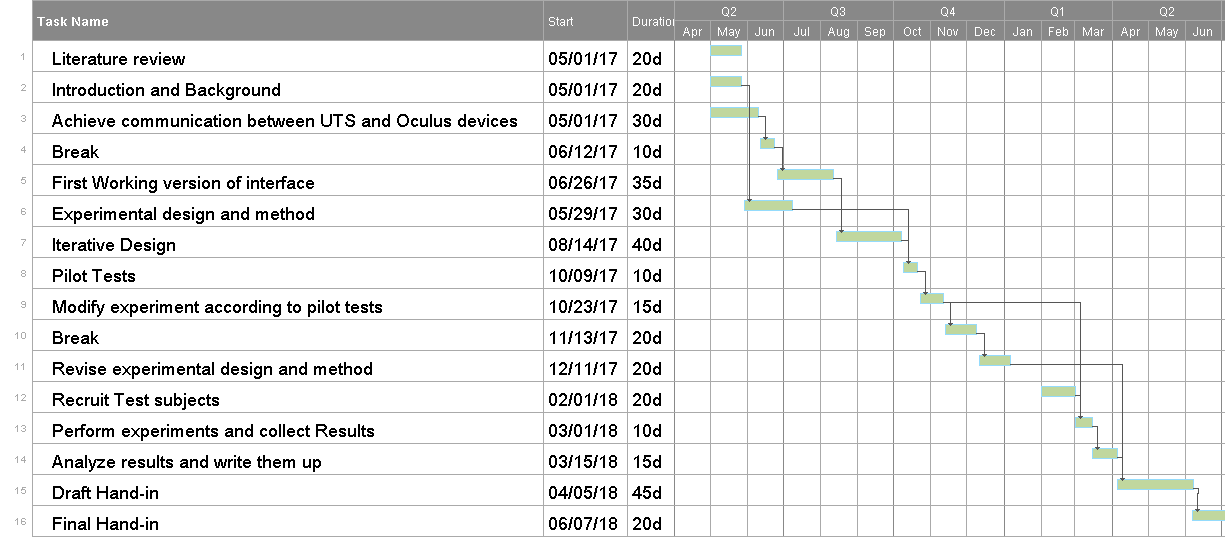
\includegraphics[width=540pt]{Gantt}
	\caption{Gantt chart Showing project goals}
\end{figure*}

\begin{table}[H]
	\centering
	\begin{tabular}{m{2cm} |m{4cm}}
		Date & Milestone\\ \hline
		01/06/2017 & Literature review, Introduction and Background complete\\
		12/06/2017 & Communication between terrain synthesis and Oculus devices\\
		14/08/2017 & First working version of software complete\\
		01/11/2017 & Iterative design and pilot tests complete \\
		15/03/2018 & Experiments Complete\\
		05/04/2018 & Results and Analysis Complete\\
		06/06/2018 & Draft hand-in\\
		01/07/2018 & Final hand-in		
	\end{tabular}
\caption{Milestones}
\end{table}
%\hl{[Make a gant chart]}
\section{Research outcomes}
\subsection{Artefacts produced}
During the course of this research a VE interface system designed for the Oculus rift and Oculus touch controllers will be developed. This will interact with the terrain synthesis functionality of the existing terrain synthesis desktop system\cite{Gain2015}. The resulting application will provide an immersive user experience that allows for terrain modelling in a VE.
\newpage
\subsection{Success factors}
It is expected that the VE interface will allow users to model terrains with a statistically significant reduction in time due to the ability to work in three dimensions. We also expect that the VE interface will provide a more natural method of interacting with the terrain model and will therefore be given a significantly higher usability rating. Due to the greater speed and more natural method of interaction we expect that users will be able to make more adjustments to their design resulting in designs that are more accurate by a statistically significant margin. By immersing designers in a VE we expect that they will gain a more realistic idea of the user experience allowing them to create designs closer to their mental models.

If these expectations are shown to be true we will be able to conclude that VE systems are advantageous over desktop interfaces for terrain modelling. 
\subsection{Relevance to industry}
Should this research show that designing VE content in VEs is viable and even advantageous it may support a move away from desktop workstations in the workplace. Additionally, although out of the scope of this project, VE interfaces may allow for effective real-time collaboration for tasks such as 3D modelling. A major concern for integrating VE designer tools into the workplace is the fatigue often associated with such devices. Even if designers are significantly faster and  more accurate in a VE this is meaningless if they cannot use it continuously for more than half an hour. Thus, while the speed and accuracy findings of this experiment will be interesting and relevant to the workplace it is the extent of user fatigue that is perhaps the most vital.
\newpage
\subsection{Further research}
As stated above one of the most exciting possibilities for research in this area lies in supporting multiple users, either locally or remotely. By giving each user a virtual avatar and the ability to naturally modify the model displayed we can create an environment that is conducive to fast, collaborative prototyping and allows for interactive presentations.
More immediately, however, further research can be done into effective ways to interact with the environment. This project, for environment interaction at least, mostly transfers the existing tools from the desktop application and makes them available in a VE. The much greater variety of interaction techniques offered by 6-DOF devices may allow for radically different interaction techniques.
\newpage
\bibliographystyle{abbrv}
\bibliography{proposal}
\end{document}